\question La gráfica de la Figura \ref{fig:escuela_pie} muestra la composición de una escuela de 2 400 personas.

\begin{minipage}{.45\textwidth}
    \begin{figure}[H]
        \centering
        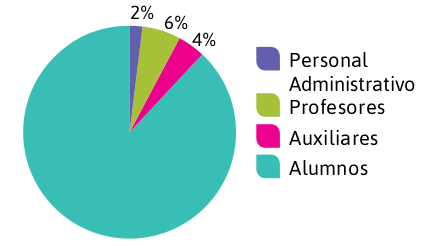
\includegraphics[width=.9\linewidth]{escuela_pie.png}
        \captionof{figure}{Gráfico circular sobre la distribución de los roles en una escuela (en porcentaje).}
        \label{fig:escuela_pie}
    \end{figure}
\end{minipage}\hfill
\begin{minipage}{.45\textwidth}
    \begin{parts}
        \part ¿Cuántas personas trabajan en la administración?
        {\printanswers
        \part ¿Cuántos profesores hay en esa escuela?

        \begin{solutionbox}{2.5cm}
            Los profesores son el 6\% de 2400, entonces:
            \[\dfrac{6}{100}\times2400=0.06\times2400=144\]
        \end{solutionbox}
        }
        \part ¿Cuántas personas son auxiliares?
        {\printanswers
        \part ¿Cuál es el porcentaje de alumnos?

        \begin{solutionbox}{2.5cm}
            El porcentaje de alumnos es::
            \[100\%-2\%-6\%-4\%=88\%\]
        \end{solutionbox}
        }
        \part ¿Cuántos alumnos tiene la escuela?
    \end{parts}
\end{minipage}
